\chapter{Experiment details for the Pixel-Wise Conditionned GAN}
\label{chap:details_neucom}
\graphicspath{{images/chapter2/}, {tikz/chapter2/} }

\section{Details of the datasets}
\label{app:det_datasets}

{
	\centering
	\begin{tabular}{|l|c|c|c|c|c|}
		\hline
		Dataset           & Size (in pixels)& Training set & Validation set & Test set\\
		\hline
		FashionMNIST &28x28& 55,000 & 5,000 & 10,000\\
		Cifar-10 & 32x32& 55,000 & 5,000 & 10,000 \\
		CelebA & 128x128 & 80,000 & 5,000 & 15,000\\
		\hline
		Texture & 160x160 & 20,000 & 2,000 & 4,000\\
		Subsurface & 160x160 & 20,000 & 2,000 & 4,000\\
		\hline
	\end{tabular}

Additional information: 

\begin{itemize}
	\item For FashionMNIST and Cifar-10, we keep the original train/test split and then sample 5000 images from the training set that act as validation samples.
	\item For the Texture dataset, we sample patches randomly from a 3840x2400 image of a brick wall.
\end{itemize}

\section{Detailed deep architectures}
\label{app:det_archis}

\subsection{DCGAN for FashionMNIST}
{
	\centering
	\begin{tabular}{|l|c|c|c|c|c|}
		\hline
		Layer type & Units & Scaling & Activation & Output shape\\
		\hline
		Input z & - & - & - & 7x7\\
		Input y & - & - & - & 28x28\\
		Dense & 343 & - & ReLU & 7x7\\
		Conv2DTranspose & 128 3x3 & x2 & ReLU & 14x14 \\
		Conv2DTranspose & 64 3x3 & x2 & ReLU & 28x28 \\
		Conv2DTranspose & 1 3x3 & x1 & tanh & 28x28 \\
		\hline
		Input x & - & - & - & 28x28\\
		Input y & - & - & - & 28x28\\
		Conv2D & 64 3x3 & x1/2 & LeakyReLU & 14x14 \\
		Conv2D & 128 3x3 & x1/2 & LeakyReLU & 7x7 \\
		Conv2D & 1 3x3 & x1 & tanh & 28x28 \\
		Dense & 1 & - & Sigmoid & 1\\
		\hline
	\end{tabular}
}\\ 

Additional information: \begin{itemize}
	\item Batch normalization \citep{Ioffe2015} is applied across all the layers
	\item A Gaussian noise is applied to the input of the discriminator
\end{itemize}

\subsection{UNet-Res for CIFAR10} \label{subsec:Unet-Cifar}
{
	\centering
	\begin{tabular}{|l|c|c|c|c|c|}
		\hline
		Layer type & Units & Scaling & Activation & Output shape\\
		\hline
		Input y & - & - & - & 32x32\\
		Conv2D* & 64 5x5 & x1 & ReLU & 32x32 \\
		Conv2D* & 128 3x3 & x1/2 & ReLU & 16x16 \\
		Conv2D* & 256 3x3 & x1/2 & ReLU & 8x8 \\
		Input z & - & - & - & 8x8\\
		Dense & 256 & - & ReLU & 8x8\\
		Residual block & 3x256 3x3 & x1 & ReLU & 8x8 \\
		Residual block & 3x256 3x3 & x1 & ReLU & 8x8 \\
		Residual block & 3x256 3x3 & x1 & ReLU & 8x8 \\
		Residual block & 3x256 3x3 & x1 & ReLU & 8x8 \\
		Conv2DTranspose* & 256 3x3 & x2 & ReLU & 16x16 \\
		Conv2DTranspose* & 128 3x3 & x2 & ReLU & 32x32 \\
		Conv2DTranspose* & 64 3x3 & x1 & ReLU & 32x32 \\
		Conv2D & 3 3x3 & x1 & tanh & 32x32 \\
		\hline
		Input x & - & - & - & 32x32\\
		Input y & - & - & - & 32x32\\
		Conv2D & 64 3x3 & x1/2 & LeakyReLU & 16x16 \\
		Conv2D & 128 3x3 & x1/2 & LeakyReLU & 8x8 \\
		Conv2D & 256 3x3 & x1/2 & LeakyReLU & 4x4 \\
		Dense & 1 & - & Sigmoid & 1\\
		\hline
	\end{tabular}
}\\ 

Additional information: \begin{itemize}
	\item Instance normalization \citep{Ulyanov2016} is applied across all the layers instead of Batch normalization. This is involved by the use of the PacGAN technique.
	\item A Gaussian noise is applied to the input of the discriminator
	\item The layers noted with an asterisk are linked with a skip-connection
\end{itemize}


\subsection{UNet-Res for CelebA}
\label{subsec:unet_celeba}
{
	\centering
	\begin{tabular}{|l|c|c|c|c|c|}
		\hline
		Layer type & Units & Scaling & Activation & Output shape\\
		\hline
		Input y & - & - & - & 128x128\\
		Conv2D & 64 5x5 & x1 & ReLU & 128x128 \\
		Conv2D* & 128 3x3 & x1/2 & ReLU & 64x64 \\
		Conv2D* & 256 3x3 & x1/2 & ReLU & 32x32 \\
		Conv2D* & 512 3x3 & x1/2 & ReLU & 16x16 \\
		Input z & - & - & - & 16x16\\
		Dense & 256 & - & ReLU & 16x16\\
		Residual block & 3x256 3x3 & x1 & ReLU & 16x16 \\
		Residual block & 3x256 3x3 & x1 & ReLU & 16x16 \\
		Residual block & 3x256 3x3 & x1 & ReLU & 16x16 \\
		Residual block & 3x256 3x3 & x1 & ReLU & 16x16 \\
		Residual block & 3x256 3x3 & x1 & ReLU & 16x16 \\
		Residual block & 3x256 3x3 & x1 & ReLU & 16x16 \\
		Conv2DTranspose* & 256 3x3 & x2 & ReLU & 32x32 \\
		Conv2DTranspose* & 128 3x3 & x2 & ReLU & 64x64 \\
		Conv2DTranspose* & 64 5x5 & x2 & ReLU & 128x128 \\
		Conv2D & 3 3x3 & x1 & tanh & 128x128 \\
		\hline
		Input x & - & - & - & 128x128\\
		Input y & - & - & - & 128x128\\
		Conv2D & 64 3x3 & x1/2 & LeakyReLU & 64x64 \\
		Conv2D & 128 3x3 & x1/2 & LeakyReLU & 32x32 \\
		Conv2D & 256 3x3 & x1/2 & LeakyReLU & 16x16 \\
		Conv2D & 512 3x3 & x1/2 & LeakyReLU & 32x32 \\
		Dense & 1 & - & Sigmoid & 1\\
		\hline
	\end{tabular}
}\\~\\
\noindent
This network follows the same additional setup as described in Appendix (\ref{subsec:Unet-Cifar}).
%Additional details: \begin{itemize}
%   \item Instance normalization\cite{ulyanov2016instance} is applied across all the layers instead of Batch normalization. This is due to the use of the PacGAN technique.
%  \item Gaussian noise is applied to the input of the discriminator
% \item The layers noted with an asterisked are linked with a skip-connection
%\end{itemize}


\subsection{Architectures for Texture}

\subsubsection{PatchGAN discriminator}
{
	\centering
	\begin{tabular}{|l|c|c|c|c|c|}
		\hline
		Layer type & Units & Scaling & Activation & Output shape\\
		\hline
		Input x & - & - & - & 160x160\\
		Input y & - & - & - & 160x160\\
		Conv2D & 64 3x3 & x1/2 & LeakyReLU & 80x80 \\
		Conv2D & 128 3x3 & x1/2 & LeakyReLU & 40x40 \\
		Conv2D & 256 3x3 & x1/2 & LeakyReLU & 20x20 \\
		Conv2D & 512 3x3 & x1/2 & LeakyReLU &  10x10\\
		\hline
	\end{tabular}
} 

\subsubsection{UpDil Texture}
{
	\centering
	\begin{tabular}{|l|c|c|c|c|c|}
		\hline
		Layer type & Units & Scaling & Activation & Output shape\\
		\hline
		Input z & - & - & - & 20x20 \\
		Conv2DTranspose & 256 3x3 & x2 & ReLU & 40x40 \\
		Conv2DTranspose & 128 3x3 & x2 & ReLU & 80x80 \\
		Conv2DTranspose & 64 3x3 & x2 & ReLU & 160x160 \\
		Input y & - & - & - & 160x160\\
		Conv2D & 64 3x3 dil. 1 & x1 & ReLU & 160x160 \\
		Conv2D & 128 3x3  dil. 2 & x1 & ReLU & 160x160 \\
		Conv2D & 256 3x3 dil. 3 & x1 & ReLU & 160x160 \\
		Conv2D & 512 3x3  dil. 4& x1 & ReLU & 160x160 \\
		Conv2D & 3 3x3 & x1 & tanh & 160x160 \\
		\hline
	\end{tabular}
}

\subsubsection{UpEncDec Texture}
{
	\centering
	\begin{tabular}{|l|c|c|c|c|c|}
		\hline
		Layer type & Units & Scaling & Activation & Output shape\\
		\hline
		Input z & - & - & - & 20x20 \\
		Conv2DTranspose & 256 3x3 & x2 & ReLU & 40x40 \\
		Conv2DTranspose & 128 3x3 & x2 & ReLU & 80x80 \\
		Conv2DTranspose & 64 5x5 & x2 & ReLU & 160x160 \\
		Input* y & - & - & - & 160x160\\
		Conv2D* & 64 3x3 & x1/2 & ReLU & 80x80 \\
		Conv2D* & 128 3x3 & x1/2 & ReLU & 40x40 \\
		Conv2D & 256 3x3 & x1/2 & ReLU & 20x20 \\
		Conv2DTranspose* & 256 3x3 & x2 & ReLU & 40x40 \\
		Conv2DTranspose* & 128 3x3 & x2 & ReLU & 80x80 \\
		Conv2DTranspose* & 64 3x3 & x2 & ReLU & 160x160 \\
		Conv2D & 3 3x3 & x1 & tanh & 160x160 \\
		\hline
	\end{tabular}
}

\subsubsection{UNet Texture}
{
	\centering
	\begin{tabular}{|l|c|c|c|c|c|}
		\hline
		Layer type & Units & Scaling & Activation & Output shape\\
		\hline
		Input y & - & - & - & 160x160\\
		Conv2D & 64 5x5 & x1 & ReLU & 160x160 \\
		Conv2D* & 128 3x3 & x1/2 & ReLU & 80x80 \\
		Conv2D* & 256 3x3 & x1/2 & ReLU & 40x40 \\
		Conv2D* & 512 3x3 & x1/2 & ReLU & 20x20 \\
		Input z & - & - & - & 20x20 \\
		Conv2DTranspose* & 256 3x3 & x2 & ReLU & 40x40 \\
		Conv2DTranspose* & 128 3x3 & x2 & ReLU & 80x80 \\
		Conv2DTranspose* & 64 5x5 & x2 & ReLU & 160x160 \\
		Conv2D & 3 3x3 & x1 & tanh & 160x160 \\
		\hline
	\end{tabular}
}

\subsubsection{Res Texture}
{
	\centering
	\begin{tabular}{|l|c|c|c|c|c|}
		\hline
		Layer type & Units & Scaling & Activation & Output shape\\
		\hline
		Input y & - & - & - & 160x160\\
		Conv2D & 64 5x5 & x1 & ReLU & 160x160 \\
		Conv2D & 128 3x3 & x1/2 & ReLU & 80x80 \\
		Conv2D & 256 3x3 & x1/2 & ReLU & 40x40 \\
		Conv2D & 512 3x3 & x1/2 & ReLU & 20x20 \\
		Input z & - & - & - & 20x20 \\
		Residual block & 3x256 3x3 & x1 & ReLU & 20x20 \\
		Residual block & 3x256 3x3 & x1 & ReLU & 20x20 \\
		Residual block & 3x256 3x3 & x1 & ReLU & 20x20 \\
		Residual block & 3x256 3x3 & x1 & ReLU & 20x20 \\
		Residual block & 3x256 3x3 & x1 & ReLU & 20x20 \\
		Residual block & 3x256 3x3 & x1 & ReLU & 20x20 \\
		Conv2DTranspose & 256 3x3 & x2 & ReLU & 40x40 \\
		Conv2DTranspose & 128 3x3 & x2 & ReLU & 80x80 \\
		Conv2DTranspose & 64 5x5 & x2 & ReLU & 160x160 \\
		Conv2D & 3 3x3 & x1 & tanh & 160x160 \\
		\hline
	\end{tabular}
} 

\subsubsection{UNet-Res Texture} 
{
	\centering
	\begin{tabular}{|l|c|c|c|c|c|}
		\hline
		Layer type & Units & Scaling & Activation & Output shape\\
		\hline
		Input y & - & - & - & 160x160\\
		Conv2D & 64 5x5 & x1 & ReLU & 160x160 \\
		Conv2D* & 128 3x3 & x1/2 & ReLU & 80x80 \\
		Conv2D* & 256 3x3 & x1/2 & ReLU & 40x40 \\
		Conv2D* & 512 3x3 & x1/2 & ReLU & 20x20 \\
		Input z & - & - & - & 20x20 \\
		Residual block & 3x256 3x3 & x1 & ReLU & 20x20 \\
		Residual block & 3x256 3x3 & x1 & ReLU & 20x20 \\
		Residual block & 3x256 3x3 & x1 & ReLU & 20x20 \\
		Residual block & 3x256 3x3 & x1 & ReLU & 20x20 \\
		Residual block & 3x256 3x3 & x1 & ReLU & 20x20 \\
		Residual block & 3x256 3x3 & x1 & ReLU & 20x20 \\
		Conv2DTranspose* & 256 3x3 & x2 & ReLU & 40x40 \\
		Conv2DTranspose* & 128 3x3 & x2 & ReLU & 80x80 \\
		Conv2DTranspose* & 64 5x5 & x2 & ReLU & 160x160 \\
		Conv2D & 3 3x3 & x1 & tanh & 160x160 \\
		\hline
	\end{tabular}
}\\~\\
\noindent
As for Cifar10, this network follows the same additional setup described in Appendix (\ref{subsec:Unet-Cifar}).

\section{Domain-specific metrics for underground soil generation}
\label{app:geostatistics}

In this section, we compute the connectivity function \cite{Lemmens2017} of generated soil image, a domain-specific metric, which is the probability that a continuous pixel path exists between two pixels of the same value (called Facies) in a given direction and a given distance (called Lag). This connectivity function should be similar to the one obtained on real-world samples. In this application, the connectivity function models the probability that two given pixels are from the same sand brick or clay matrix zone.

\begin{figure}[t]
	\centering
	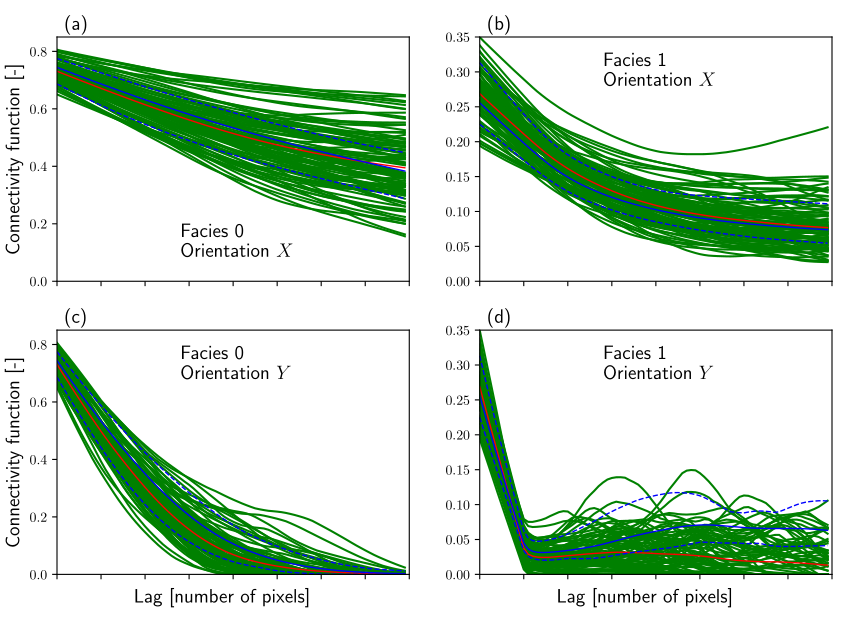
\includegraphics[scale=0.45]{out_cgan_Connect_edited.png}
	\caption{Connectivity curves obtained on 100 samples generated with the CGAN approach.}
	\label{fig:CGAN_connectivity}
\end{figure}

\begin{figure}[!t]
	\centering
	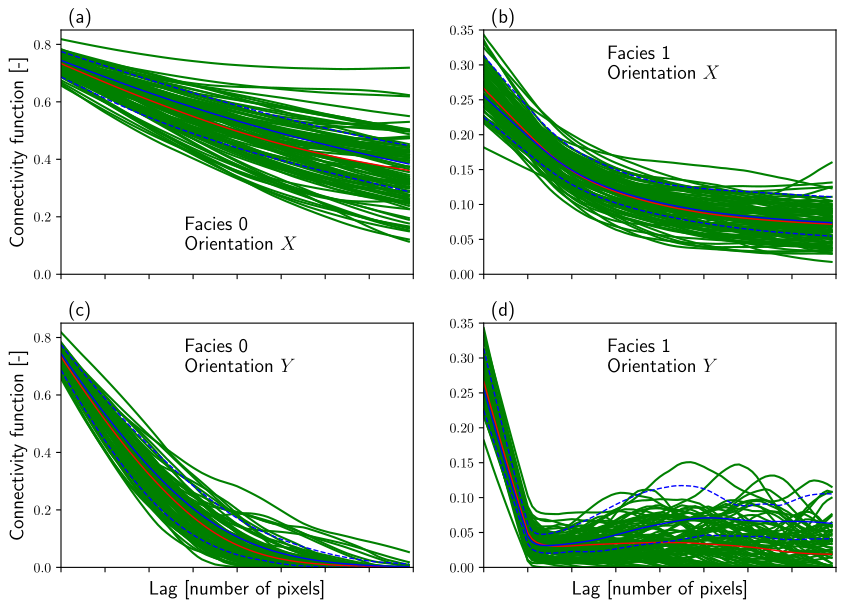
\includegraphics[scale=0.45]{out_neurocomp_Connect_edited.png}
	\caption{Connectivity curves obtained on 100 samples generated with our approach.}
	\label{fig:ours_connectivity}
\end{figure}



We sampled 100 real and 100 generated images using the UNetResPAC architecture (see Section \ref{subs:architectures}) on which the connectivity function was evaluated for both the CGAN and our approach. The obtained graphs are shown respectively in Figures \ref{fig:CGAN_connectivity} and \ref{fig:ours_connectivity}.

The blue curves are the mean value for the real samples, and the blue dashed curves are the minimum and maximum values on these samples. The green curves are the connectivity functions for each of the 100 synthetic samples and the red curves are their mean connectivity functions.
%
From these curves
%the Figures \ref{fig:CGAN_connectivity} and \ref{fig:ours_connectivity}, 
we observe that that our approach has similar connectivity functions as the CGAN approach while being significantly better at respecting the given constraints (see Section Table \ref{tab:subsurface}). 
